The \textit{Degree matrix} \(D\) is a diagonal matrix that has the degree of each node on the diagonal where the degree of a node \(v_i\) is the sum of the weights of all the edges that are connected to such node. Since in our case edge weights correspond to similarities, the degree of each node is the sum of the similarities with all of its neighbors. This can be simply achieved with the following:
\begin{equation}
    D = \text{diag}(W \mathbbm{1})
\end{equation}
Since the Laplacian matrix is defined as \(L= D - W\), we use the following code to compute both \(D\) and \(L\):
\lstinputlisting{../graph_laplacian.m}
After computing Both matrices for each dataset and for each value of \(K\) we are testing for the K-NN graph we can inspect each Laplacian matrix using the \texttt{spy} command in MATLAB:
\begin{figure}[H]
    \centering
    \subfloat[1][\(K= 10\)]{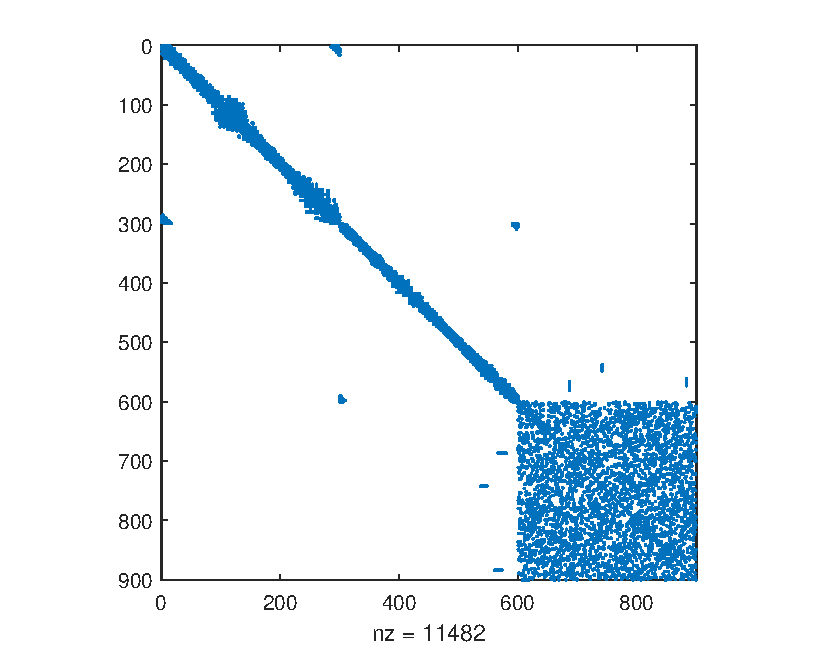
\includegraphics[scale = 0.37]{pictures/circle_LaplacianSpy_K10.pdf}}
    \subfloat[2][\(K= 20\)]{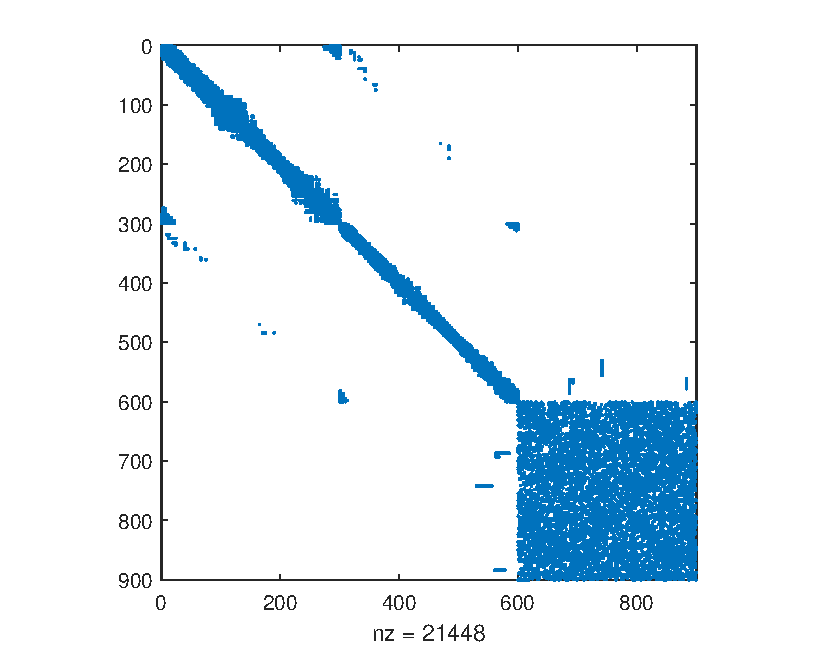
\includegraphics[scale = 0.37]{pictures/circle_LaplacianSpy_K20.pdf}}
    \subfloat[3][\(K= 40\)]{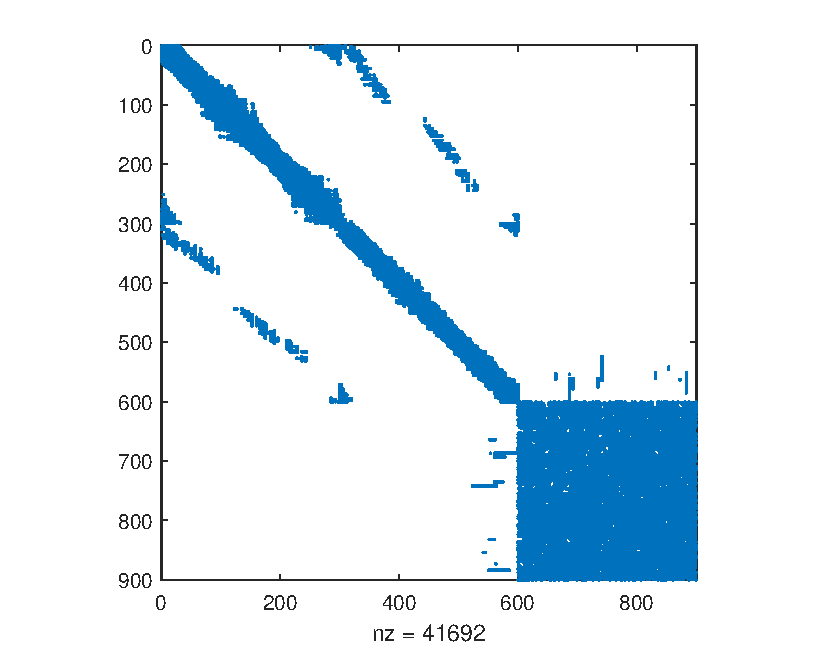
\includegraphics[scale = 0.37]{pictures/circle_LaplacianSpy_K40.pdf}}
    \caption{\texttt{spy} plots of the Laplacian matrix for \texttt{Circle} data with different values of \(K\)}
    \label{LaplacianSpy_circle}
  \end{figure}
  In Figure \ref{LaplacianSpy_circle} we can see that, for each Laplacian matrix inspected, there are 3 sections. Each section defines a "\textit{shape cluster}" in the \texttt{Circle} dataset: the first one is clearly vidible in the bottom right corner of each matrix and it is relative to the point cloud. The other two sections are along the diagonal in the top left of the matrix, they are somewhat visible for \(K= 10\) and \(K= 20\) and they are relative to the two "circles" visible in the scatterplot in Figure \ref{scatter_intro}. The Laplacian matrix inspected for \(K= 40\) clearly shows a sort of \textbf{data pollution} from one shape cluster to another, this might suggest that the value \(K= 40\) may be too high for deploying the clustering.
  \begin{figure}[H]
    \centering
    \subfloat[1][\(K= 10\)]{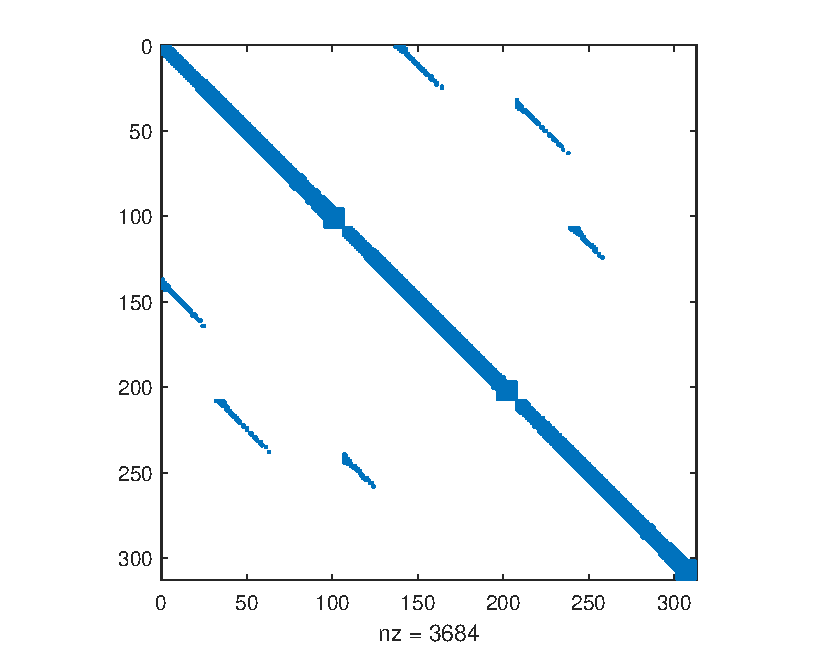
\includegraphics[scale = 0.37]{pictures/spiral_LaplacianSpy_K10.pdf}}
    \subfloat[2][\(K= 20\)]{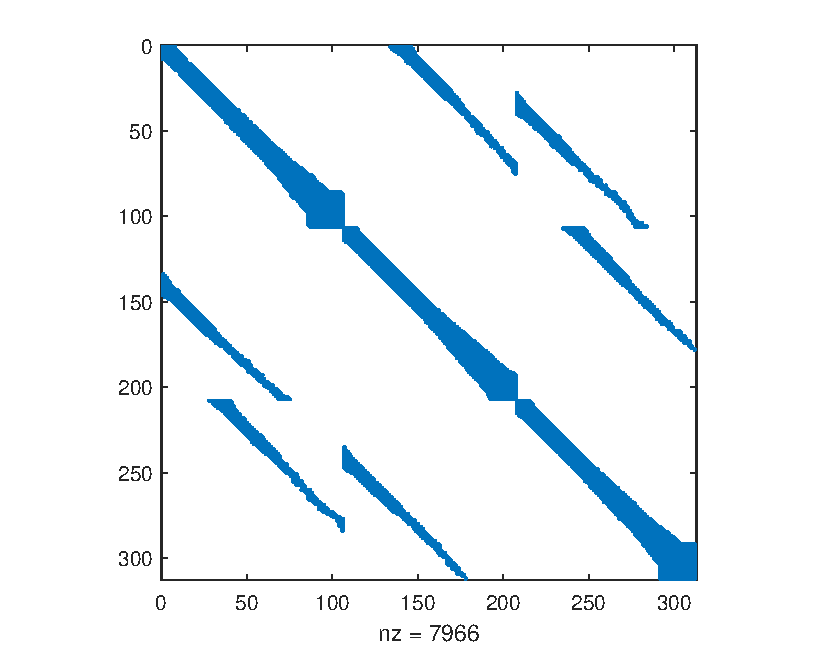
\includegraphics[scale = 0.37]{pictures/spiral_LaplacianSpy_K20.pdf}}
    \subfloat[3][\(K= 40\)]{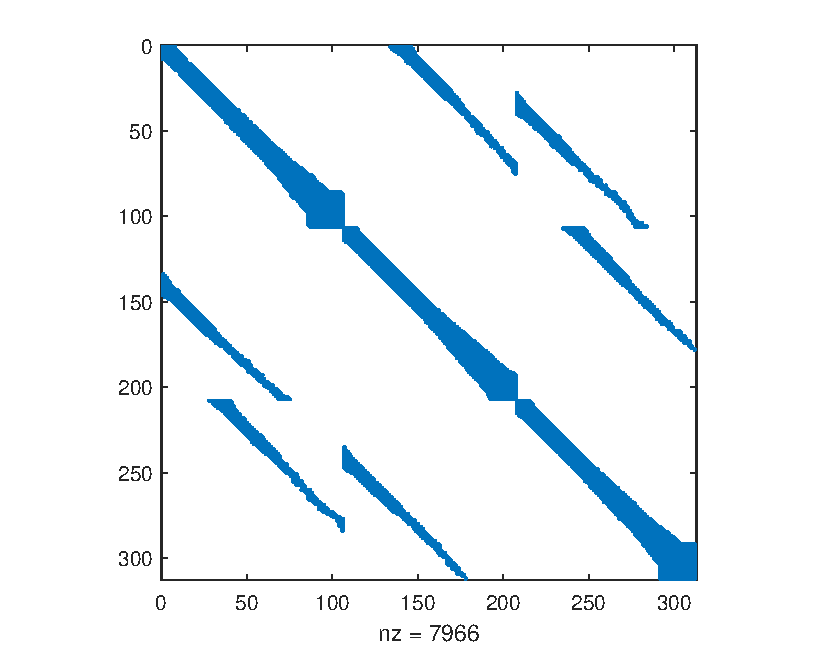
\includegraphics[scale = 0.37]{pictures/spiral_LaplacianSpy_K20.pdf}}
    \caption{\texttt{spy} plots of the Laplacian matrix for \texttt{Spiral} data with different values of \(K\)}
    \label{LaplacianSpy_spiral}
  \end{figure}
  The same concept can be applied for Figure \ref{LaplacianSpy_spiral}. Along the diagonal, three sections are visible and they represent the three different spirals seen in Figure \ref{scatter_intro}. As for \texttt{Circle} data, the KNN graph computed on the \texttt{Spiral} data with \(K= 40\) shows pollution between each spiral and this is visibile since there are a lot of non-zero elements away from the diagonal.
  \\
\\
The recurrent theme for both dataset is that the more \(K\) is higher, the more each shape will "pollute" another. This means that the corresponding Laplacian matrix will show a \textbf{lot of non-zero elements away from the diagonal} and this is a phenomenon that can (and will) impact computational costs.